% !TeX root = ../main.tex
% Add the above to each chapter to make compiling the PDF easier in some editors.

\chapter{Seissmic Waves and ADER-DG formulation}\label{chapter:seismicwaves}
In this chapter, we establish the theoretical foundations necessary for this thesis by deriving the fundamental equations for elastic
wave propagation and presenting the equation of motion in velocity-stress formulation. We assume isotropic media and utilize symmetry arguments
throughout the work. The restriction to isotropic media is a commonly employed simplification, as seen in works such as ~\parencite{dumbser1}. \\

The next section of the thesis discusses SeisSol, the numerical tool employed for simulating seismic wave phenomena. SeisSol is a combination
of the \ac{DG-FE} method and a time integration scheme based on the solution of \ac{ADER}, as described in previous works ~\parencite{dumbser1}, ~\parencite{seissol}. This approch, known as 
\ac{ADER}-\ac{DG} will be introduced in more detail in the following sections.

\section{Elastic Wave Equation}\label{section:elasticwaveequation}
An elastic medium is characterized by an undeformed state, in which stresses and strains are zero, to which it will return to in the absence
of outer forces. If the stresses and strains the medium experiences are infinitesimal, the theory of linear elasticity applies. We define
the displacement vector $\mathbf{U}$ describing the shortest distance between the initial and current position of a point. The particle
velocities $u,v$ and $w$ in $x, y, z$ direction, respectively, can then be defined as the temporal derivate of $\mathbf{U}$

\begin{align}
    \begin{split}
    \frac{\partial U_x}{\partial t} = \dot{U}_x = u \\
    \frac{\partial U_y}{\partial t} = \dot{U}_y = v \\
    \frac{\partial U_z}{\partial t} = \dot{U}_z = w, \\
    \end{split}
 \end{align}

where the subscript denotes the coordinate direction and a dot over a variable represents its partial time derivative leading to the following notation:

\begin{align}
    \begin{split}
        \frac{\partial U_i}{\partial t} = \partial_t U_i = \dot{U}_i = V_i,
    \end{split}
    \label{equation1}
\end{align}

where the velocity vector \textbf{V} is introduced. \\

In the context of linear elasticity, the following extension of Hooke's law holds

\begin{align}
    \begin{split}
        \sigma_{ij} = c_{ijkl}\epsilon_{kl},
    \end{split}
    \label{eq:hookeslaw}
\end{align}

with the medium specific constants $c_{ijkl}$ being used to generalize Hooke's law in linear elasticity. The Einstein summation convention
is followed, where an index appearing twice is summed over all possible values. In this context, $\sigma_{ij}$ represents the stress tensor
and $\epsilon_{kl}$ represents the strain tensor. Hooke's law expresses that stress tensor components are linear combinations of strain tensor
components. For infinitesimally small perturbations, the strain tensor components $\epsilon_{kl}$ are defined as follows

\begin{align}
    \begin{split}
        \epsilon_{kl} = \frac{1}{2}\left(\partial_k U_l + \partial_l U_k \right) ,
    \end{split}
\end{align}

where $\partial_k$ represents the spatial derivative in k-direction and $U_i$ represents the displacement in i-direction.
Previously, we mentioned our focus on the velocity-stress formulation rather than the displacement-stress formulation.
To eliminate the displacements $U_i$, we introduced velocities $V_i$ in equation \ref{equation1}.
Consequently, this leads to the time derivative of the strain tensor

\begin{align}
    \begin{split}
        \dot{\epsilon}_{kl} = \frac{1}{2}\left( \partial_k V_l + \partial_l V_k \right) ,
    \end{split}
\end{align}

expressed in terms of the spatial derivatives of the velocities $V_i$. It is straightforward to calculate the time derivative
of the stress tensor if the constants $c_{ijkl}$ remain constant over time

\begin{align}
    \begin{split}
        \dot{\sigma}_{ij} = c_{ijkl}\dot{\epsilon}_{kl} .
    \end{split}
    \label{eq:stress}
\end{align}

We can apply symmetry considerations to the term $c_{ijkl}$ in equation \ref{eq:hookeslaw} and reduce the number of independent components from 81 to 21(~\parencite{aki2002quantitative} Chapter 2).
This in turn lets us define the tensor in terms of two constants in isotropic media with the general form of

\begin{equation}
    c_{ijkl} = \lambda \delta_{ij}\delta_{kl} + \mu\left(\delta_{ik}\delta_{jl} + \delta_{il}\delta_{jk}\right),
    \label{eq:isotropic}
\end{equation}

where $\delta$ is the Kronecker-delta function and $\lambda, \mu$ are the Lam\'e parameters. \\

We now write a force balance in a volume $V$ within a surface $S$. The momentum within the volume changes at a rate equal
to the forces acting on that volume. Therefore, the forces acting on these comprise a body force and a surface force, which result
from the presence of normal and shear stresses. This can be written mathematically as 

\begin{equation}
    \frac{\partial}{\partial t} \int_V \rho \frac{\partial \mathbf{U}}{\partial t}dV = \int_V \mathbf{f}dV + \oint_S \mathbf{T\left(n\right)}dS,
    \label{eq:forcebalance}
\end{equation}

where $\frac{\partial}{\partial t} \int_V \rho \frac{\partial \mathbf{U}}{\partial t}dV$, is the momentum of the control volume with density $\rho$, and $\mathbf{T}$
is the traction vector which is related to the stress tensor by Cauchy's stress theorem ~\parencite{cauchy-stress-theorem}

\begin{equation}
    T_j\left(n\right) = \sigma_{ij}n_i,
\end{equation}

with the normal vector $n_i$. Replacing $\mathbf{T}$ in \refeq{eq:forcebalance} using the above
,applying Gauss' divergence theorem and reshuffling gives us

\begin{equation}
    \int_V \left(\rho \ddot{U}_i - f_i - \partial_j \sigma_{ij}\right)dV = 0.
\end{equation}

Here we assumed that the stress tensor is symmetric, i.e., $\sigma_{ij}=\sigma_{ji}$. As it is true for any general volume, we can
equate the integrand to zero. This gives us the equation

\begin{equation}
    \rho \ddot{U}_i = f_i + \partial_j \sigma_{ij},
    \label{eq:force}
\end{equation}

expanding it in $j$ and using $V_i = \frac{\partial U_i}{\partial t}$,

\begin{equation}
    \rho \frac{\partial V_i}{\partial t} = f_i + \partial_x \sigma_{xi} + \partial_y \sigma_{yi} + \partial_z \sigma_{zi},
    \label{eq:finalequation}
\end{equation}

The body force $f_i$ will be discussed later in terms of the source terms. \\

Combining equations \ref{eq:stress}, \ref{eq:isotropic}, \ref{eq:finalequation}, we obtain the final 3D 
wave elastic equation for an isotropic medium in velocity-stress formulation

\begin{align}
    \begin{split}
    \frac{\partial \sigma_{xx}}{\partial t} - \left(\lambda  + 2\mu\right)\frac{\partial u}{\partial x} - \lambda \frac{\partial v}{\partial y} - \lambda\frac{\partial w}{\partial z} &= S_1, \\    
    \frac{\partial \sigma_{yy}}{\partial t} - \lambda \frac{\partial u}{\partial x} - \left( \lambda + 2 \mu \right)\frac{\partial v}{\partial y} - \lambda \frac{\partial w}{\partial w} &= S_2, \\
    \frac{\partial \sigma_{zz}}{\partial t} - \lambda \frac{\partial u}{\partial x} - \lambda \frac{\partial v}{\partial y} - \left(\lambda + 2\mu\right)\frac{\partial w}{\partial z} &= S_3, \\
    \frac{\partial \sigma_{xy}}{\partial t} - \mu \left(\frac{\partial v}{\partial x} + \frac{\partial u}{\partial y}\right) &= S_4, \\ 
    \frac{\partial \sigma_{yz}}{\partial t} - \mu \left(\frac{\partial v}{\partial z} + \frac{\partial w}{\partial y}\right) &= S_5, \\
    \frac{\partial \sigma_{xz}}{\partial t} - \mu \left(\frac{\partial u}{\partial z} + \frac{\partial w}{\partial x}\right) &= S_6, \\
    \rho \frac{\partial u}{\partial t} - \frac{\partial \sigma_{xx}}{\partial x} - \frac{\partial \sigma_{xy}}{\partial y} - \frac{\partial \sigma_{xz}}{\partial z} &= \rho S_7, \\
    \rho \frac{\partial v}{\partial t} - \frac{\partial \sigma_{xy}}{\partial x} - \frac{\partial \sigma_{yy}}{\partial y} - \frac{\partial \sigma_{yz}}{\partial z} &= \rho S_8, \\
    \rho \frac{\partial w}{\partial t} - \frac{\partial \sigma_{xz}}{\partial x} - \frac{\partial \sigma_{yz}}{\partial y} - \frac{\partial \sigma_{zz}}{\partial z} &= \rho S_9, \\
\end{split}
\label{eq:setofequations}
\end{align}

where $S_p, p = 1,\dots9,$ are the source terms. \\

Another important term for consideration with this system is the propagation speed of elastic-acoustic waves. In elastic media, we will 
observe two kinds of waves, a primary compression wave and a secondary sheer wave which are called P-waves and S-waves respectively.\\

Inserting the definition of stress $\sigma_{ij}$ from equation \ref{eq:hookeslaw} and $c_{ijkl}$ from equation \ref{eq:isotropic} into equation \ref{eq:force},
we obtain when there are no external sources

\begin{equation}
    \rho \ddot{U}_i = \left(\lambda + \mu \right)\partial_i \partial_j u_j + \mu \partial_j \partial_j u_i.
    \label{eq:einsteinconvention}
\end{equation}

We use a vector relation,

\begin{equation}
    \nabla \times \left(\nabla \times \mathbf{U}\right) = \nabla\left(\nabla \cdot \mathbf{U}\right) - \nabla^2 \mathbf{U}
\end{equation}

to convert equation \ref{eq:einsteinconvention} into a vector equation. Combining these two we get:

\begin{align}
    \begin{split}
        \rho \ddot{\mathbf{U}} &= \left(\lambda + \mu\right)\nabla\left(\nabla\cdot\mathbf{U}\right) + \mu \nabla^2 \mathbf{U} \\
        &= \left(\lambda + \mu\right)\nabla\left(\nabla \cdot \mathbf{U}\right) - \mu \nabla \times \left(\nabla \times \mathbf{U}\right) + \mu \nabla\left(\nabla \cdot \mathbf{U}\right) \\
        \rho \ddot{\mathbf{U}} &= \left(\lambda + 2\mu\right)\nabla\left(\nabla\cdot\mathbf{U}\right) - \mu \nabla\times\left(\nabla\times\mathbf{U}\right). 
    \end{split}
    \label{eq:vectorequation}
\end{align}

~\Parencite[Sec. 2.1]{kaufman} explains the characterisation and the two different wave speeds related to the equation \ref{eq:vectorequation} as

\begin{equation}
    v_p = \sqrt{\frac{\lambda + 2\mu}{\rho}}, v_s = \sqrt{\frac{\mu}{\rho}}.
    \label{eq:wavevelocities}
\end{equation}

These two velocities are the propagation velocities with $v_p$ as the propagation velocity of the P-wave and $v_s$ as the propagation velocity of the S-wave. \\

We get only one propagating wave when we set $\mu = 0$ with $v_p = \sqrt{\frac{\lambda}{\rho}}$ and simplifies the elastic wave propagation to an acoustic case.
We start our time reversal by reversing an acoustic wave(put reference to the section here) and then move on to the elastic case. Further simplifications like 

\begin{equation}
    \sigma_{ij} = 0, \forall i \neq j
\end{equation}

can be derived from the set of equations \ref{eq:setofequations}. All the diagonal elements $\sigma_{ii} = \lambda \partial_j u_j$
are equal to each other which is analogous to the physical pressure in acoustic media. 

\begin{equation}
    p \eqcolon \sigma_{xx} = \sigma_{yy} = \sigma_{zz} = \lambda \partial_iu_i,
\end{equation}

where Einstein summation is used to condense the equation. And the equation of motion condenses to

\begin{equation}
    \rho \frac{\partial^2 \mathbf{U}_i}{\partial t^2} - \partial_i p = 0.
\end{equation}

\section{\ac{ADER}-\ac{DG}}\label{section:ADER-DG}

In this section, we will discuss on the fundamental framework of SeisSol, which is the \ac{ADER}-\ac{DG} method. This section is to provide
a brief understanding about the framework and not to go too much into detail. Interested readers are redirected to ~\parencite{martin}, ~\parencite{Toro2002},~\parencite{dumbser1}, ~\parencite{DUMBSER2005683}, ~\parencite{Toro2001}, ~\parencite{seissol}.

\subsection[Discontinuous Galerkin method]{Discontinuous Galerkin Method}\label{subsection:DG}

We have earlier formulated the elastic wave equation as a system of linear hyperbolic partial differential equataions. ~\parencite{osti_4491151}
first used the \ac{DG-FE} to solve these kind of problems numerically. ~\parencite{Toro2001} formulated the idea of arbitrary high order generalized
Riemann Solvers in a finite volume framework and coined the approach \ac{ADER}. Here, the combination of the generalized Riemann Solvers with \ac{DG}
methods is explained, resulting in \ac{ADER}-\ac{DG} approach (~\parencite{Dumbser2006}). Higher-order piecewise polynomial approximations are used
along with the theory of fluxes across element boundaries from the finite volume methods. The \ac{ADER}-\ac{DG} scheme is an explicit one step scheme.
It advances the solution by a full time step and needs the computation of inter-cell fluxes once per time-step. \\
% Time Derivatives are replaced with space derivatives
% using Cauchy-Kowalevski or Lax-Wendroff procedure to achieve arbitrary high-order accuracy in both space and time.

To solve the 3D elastic wave equation with the \ac{ADER}-\ac{DG} method, we need to transform it into a more compact form of hyperbolic equations

\begin{equation}
    \frac{\partial Q_p}{\partial t} + A_{pq} \frac{\partial Q_q}{\partial x} + 
    B_{pq} \frac{\partial Q_q}{\partial y} + C_{pq} \frac{\partial Q_q}{\partial z} = 0,
    \label{eq:compactform}
\end{equation}

where $\mathbf{Q}$ is the state vector with p unknown variables which contains the stresses and velocities, i.e.,

\begin{equation}
    \mathbf{Q} = \left(\sigma_{xx}, \sigma_{yy}, \sigma_{zz}, \sigma_{xy}, \sigma_{yz}, \sigma_{xz}, u, v, w \right)^T
\end{equation}

and $A_{pq}, B_{pq}, C_{pq}$ are space-dependent Jacobian matrices. Where

\begin{align}
    \begin{split}
    A_{pq} = 
        \begin{bmatrix}
        0 & 0 & 0 & 0 & 0 & 0 & -\left(\lambda + 2\mu\right) & 0 & 0 \\
        0 & 0 & 0 & 0 & 0 & 0 & -\lambda                     & 0 & 0 \\
        0 & 0 & 0 & 0 & 0 & 0 & -\lambda                     & 0 & 0 \\
        0 & 0 & 0 & 0 & 0 & 0 & 0                   & -\mu & 0 \\
        0 & 0 & 0 & 0 & 0 & 0 & 0                   & 0 & 0 \\
        0 & 0 & 0 & 0 & 0 & 0 & 0                   & 0 & -\mu \\
        -\frac{1}{\rho} & 0 & 0 & 0 & 0 & 0 & 0                   & 0 & 0 \\
        0 & 0 & 0 & -\frac{1}{\rho} & 0 & 0 & 0                   & 0 & 0 \\
        0 & 0 & 0 & 0 & 0 & -\frac{1}{\rho} & 0                   & 0 & 0 \\
    \end{bmatrix},
    \end{split}
    \label{eq:fluxmatrix}
\end{align}

and matrices $B_{pq}, C_{pq}$ are essentially similar with non-zero entries rotated around. Interested readers can refer to
~\parencite{dumbser1} for all the three matrices explicitly stated. \\

As we are dealing with unstructured meshes, we divide our computational domain $\Omega \in \mathbb{R}^3$ into tetrahedral elements 
$\mathcal{T}^{\left(m\right)}$, with unique indices $m\in\mathbb{N}$. $A_{pq}, B_{pq}, C_{pq}$ are assumed to be piecewise constant
inside each tetrahedron. We now introduce a new coordinate system of $\left(\xi, \eta, \zeta \right)$ with the frame of reference as our tetrahedron as shown 
in figure \ref{fig:transformation} \\

\begin{figure}
    \centering
    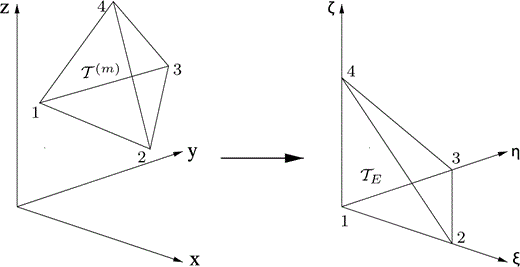
\includegraphics[width=0.6\linewidth]{figures/m_167-1-319-fig001.png}
    \caption{Tranforming tetrahedron into a reference frame.(Figure taken from Figure 1 in ~\parencite{dumbser1})}
    \label{fig:transformation}
\end{figure}

As we are dealing with a new transformed coordinate system, we would need a Transformation matrix to transform the vector $Q_p$
from the global Cartesian system to the vector $Q_q^n$ in the normal, face-aligned frame. The transformation would be of the form

\begin{equation}
    Q_p = T_{pq}Q_q^n .
\end{equation}

~\parencite{dumbser1} calculates the transformation matrix $T_{pq}$ as

\begin{align}
    \begin{split}
    T_{pq} = 
        \begin{bmatrix}
        n_x^2 & s_x^2 & t_x^2 & 2n_x s_x & 2s_x t_x & 2n_x t_x & 0 & 0 & 0 \\
        n_y^2 & s_y^2 & t_y^2 & 2n_y s_y & 2s_y t_y & 2n_y t_y & 0 & 0 & 0 \\
        n_z^2 & s_z^2 & t_z^2 & 2n_z s_z & 2s_z t_z & 2n_z t_z & 0 & 0 & 0 \\
        n_y n_x & s_y s_x & t_y t_x & n_y s_x + n_x s_y & s_y t_x + s_x t_y & n_y t_x + n_x t_y & 0 & 0 & 0 \\
        n_z n_y & s_z s_y & t_z t_y & n_z s_y + n_y s_z & s_z t_y + s_y t_z & n_z t_y + n_y t_z & 0 & 0 & 0 \\
        n_z n_x & s_z s_x & t_z t_x & n_z s_x + n_x s_z & s_z t_x + s_x t_z & n_z t_x + n_x t_z & 0 & 0 & 0 \\
        0 & 0 & 0 & 0 & 0 & 0 & n_x & s_x & t_x \\
        0 & 0 & 0 & 0 & 0 & 0 & n_y & s_y & t_y \\
        0 & 0 & 0 & 0 & 0 & 0 & n_z & s_z & t_z \\
    \end{bmatrix},
    \end{split}
\end{align}

where $\mathbf{n} = \left(n_x, n_y, n_z\right)^T$ are the components of the normal vector, and $\mathbf{s} = \left(s_x, s_y, s_z\right)^T$ and
$\mathbf{t} = \left(t_x, t_y, t_z\right)^T$ are the tangential vectors of the boundary face of the tetrahedron. $\mathbf{n}, \mathbf{s}, \mathbf{t}$
are orthogonal to each other. Mapping the physical coordinates $\left(x, y, z\right)$ with the reference element $\left(\xi, \eta, \zeta\right)$

\begin{equation}
    Q_p^{\left(m\right)} \left(x,y,z,t\right) = \hat{Q}_{pl}^{\left(m\right)} \left(t\right) \Psi_l \left(x, y, z\right),
    \label{eq:mapping}
\end{equation}

where $\Psi_l\left(x,y,z\right)$ are spatial polynomial basis functions defined on the physical element. We express \ref{eq:mapping} in 
the frame of the reference element using a suitable coordinate transformation M

\begin{equation}
     Q_p^{\left(m\right)}\left(x,y,z,t\right) = \hat{Q}_{pl}^{\left(m\right)}\left(t\right) \Psi_l\left(M\left(\xi, \eta, \zeta\right)\right).
\end{equation}

This formulation allows us to define the polynomial basis functions on the reference element $\Phi_l\left(\xi, \eta, \zeta\right)$.
As we can compute the integrals in the reference system beforehand, the coordinate transformation makes our implementation more computationally
efficient. To represent the numerical solution $Q_h$ as a linear combination of pure spatial and pure time dependent functions, we introduce
the time-dependent degrees of freedom $\hat{Q}_m\left(t\right)$. This allows us to express $Q_h$ in each tetrahedron as 

\begin{equation}
    \left[Q_H^{\left(m\right)}\right]_p \left(\xi, \eta, \zeta, t\right) = \hat{Q}_{pl}^m \left(t\right) \Phi_l \left(\xi, \eta. \zeta\right),
\label{eq:solution}
\end{equation}

where $l$ denotes the $l^{th}$ basis function. Multiplying equation \ref{eq:compactform} with the test function $\Psi_k$(~\parencite{cockburn2011discontinuous})
and integrating over our tetrahedral element $\mathcal{T}^{\left(m\right)}$ gives

\begin{equation}
    \int_{\mathcal{T}^{\left(m\right)}} \Psi_k \frac{\partial Q_p}{\partial t} dV + \int_{\mathcal{T}^{\left(m\right)}} \Psi_k \left(A_{pq} 
    \frac{\partial Q_q}{\partial x} + B_{pq}\frac{\partial Q_q}{\partial y} + C_{pq}\frac{\partial Q_q}{\partial z}\right)dV = 0,
\end{equation}

in the weak form. We add fluxes $F_p^h$ at the boundaries of the tetrahedron to include discontinuities in $Q_h$ and we integrate by parts 

\begin{equation}
    \int_{\mathcal{T}^{\left(m\right)}} \Psi_k \frac{\partial Q_p}{\partial t} dV + \int_{\partial \mathcal{T}^{\left(m\right)}} F_p^h dS
    - \int_{\mathcal{T}^{\left(m\right)}} \left(\frac{\partial \Psi_k}{\partial x} A_{pq}Q_q + \frac{\partial \Psi_k}{\partial y}B_{pq}Q_q
    + \frac{\partial \Psi_k}{\partial z}C_{pq}Q_q\right) dV = 0.
\label{eq:weakformulation}
\end{equation}

The flux between the tetrahedron $\mathcal{T}^{\left(m\right)}$ with the boundary extrapolated numerical solution $\hat{Q}_{sl} \Psi_l^{\left(m\right)}$
and one of its neighboring tetrahedra $\mathcal{T}^{\left(m_j\right)} \left(j=1,2,3,4\right)$ is computed in the global, coordinate system using the Jacobian
matrix $A_{pq}$ from equation \ref{eq:fluxmatrix}

\begin{equation}
    F_p^h = \frac{1}{2} T_{pq} \left(A_{qr}^{\left(m\right)} + \left|A_{qr}^{\left(m\right)}\right|\right)\left(T_{rs}\right)^{-1}
    \hat{Q}_{sl}^{\left(m\right)} \Psi_l^{\left(m\right)} + \frac{1}{2}T_{pq}\left(A_{qr}^{\left(m\right)} - \left|A_{qr}^{\left(m\right)}\right|\right)
    \left(T_{rs}\right)^{-1}\hat{Q}_{sl}^{\left(m_j\right)}\Psi_l^{\left(m_j\right)},
    \label{eq:fluxcalculation}
\end{equation}

where

\begin{equation}
\left|A_{qr}^{\left(m\right)}\right| = R_{qp}^A \left|\Lambda_{ps}\right| \left(R_{sr}\right)^{-1},
\end{equation}
    
and $\Lambda$ is the diagonal matrix with eigenvalues of $A_{pq}$ and $R_{pq}$ with right eigenvectors of $A_{pq}$ stacked in columns.
The next step would be inserting fluxes from equation \ref{eq:fluxcalculation} and $Q_h$ from equation \ref{eq:solution} into the weak
formulation in equation \ref{eq:weakformulation}. But as the basis functions $\Phi_l$ are defined in $\left(\xi, \eta, \zeta\right)$, we need
to transform the resulting equation with the transformation

\begin{equation}
    dx dx dz = \left|J\right| d\xi d\eta d\zeta,
\end{equation}

and linear combination of the Jacobians to create transformed Jacobian matrices

\begin{align}
    \begin{split}
        A_{pq}^{*} &= A_{pq} \frac{\partial \xi}{\partial x} + B_{pq} \frac{\partial \xi}{\partial y} + C_{pq} \frac{\partial \xi}{\partial z}, \\
        B_{pq}^{*} &= A_{pq} \frac{\partial \eta}{\partial x} + B_{pq} \frac{\partial \eta}{\partial y} + C_{pq} \frac{\partial \eta}{\partial z}, \\ 
        C_{pq}^{*} &= A_{pq} \frac{\partial \zeta}{\partial x} + B_{pq} \frac{\partial \zeta}{\partial y} + C_{pq} \frac{\partial \zeta}{\partial z}. 
    \end{split}
\end{align}

We finally get the semi-discrete \ac{DG} formulation of the ODE system within the reference tetrahedron $\mathcal{T}_E$

\begin{align}
    \begin{split}
        & \frac{\partial \hat{Q}_{pl}^{\left(m\right)}}{\partial t} \left|J\right| \int_{\mathcal{T}_E} \Phi_k \Phi_l d\xi d\eta d\zeta \\
        & + \sum_{j=1}^4 T_{pq}^j \frac{1}{2} \left(A_{qr}^{\left(m\right)} + \left| A_{qr}^{\left(m\right)}\right| \right) \left(T_{rs}^j\right)^{-1} \hat{Q}_{sl}^{\left(m\right)} \left|S_j\right| F_{kl}^{-,j} \\
        & + \sum_{j=1}^4 T_{pq}^j \frac{1}{2} \left(A_{qr}^{\left(m\right)} - \left| A_{qr}^{\left(m\right)}\right| \right) \left(T_{rs}^j\right)^{-1} \hat{Q}_{sl}^{\left(m_j\right)}\left|S_j\right| F_{kl}^{+,j,i,h} \\ 
        & - A_{pq}^* \hat{Q}_{ql}^{\left(m\right)} \left|J\right| \int_{\mathcal{T}_E} \frac{\partial \Phi_k}{\partial \xi} \Phi_l d\xi d\eta d\zeta
        - B_{pq}^* \hat{Q}_{ql}^{\left(m\right)} \left|J\right| \int_{\mathcal{T}_E} \frac{\partial \Phi_k}{\partial \eta} \Phi_l d\xi d\eta d\zeta
        - C_{pq}^* \hat{Q}_{ql}^{\left(m\right)} \left|J\right| \int_{\mathcal{T}_E} \frac{\partial \Phi_k}{\partial \zeta} \Phi_l d\xi d\eta d\zeta = 0,
    \end{split}
    \label{eq:finalform}
\end{align}

where $\left|S_j\right|$ is the area of the face $j$ of the tetrahedron.

\subsection[ADER Time Discretization]{ADER Time Discretization}

Instead of now utilizing the Runge-Kutta method to derive a limited fourth-order in time Runge-Kutta \ac{DG} scheme, we adopt the 
\ac{ADER} approach to achieve an arbitrary high-order accuracy in both spatial and temporal dimensions. Runge-Kutta schemes of order
higher than 4 tend to become inefficient as the number of calculation steps required exceeds the order of accuracy due to the Butcher barriers(~\parencite{butcher1987numerical}). \\

By applying the \ac{ADER} scheme to the \ac{DG} formulation described in equation \ref{eq:finalform}, we obtain the \ac{ADER}-\ac{DG} scheme.
The crucial step in this approach involves using the Cauchy-Kovalewski procedure to replace time-derivatives with pure space derivatives.
As a consequence, the Cauchy-Kovalewski procedure provides the $k^{th}$ time-derivative as shown in equation \ref{eq:cauchy-kovalewski} in the face-aligned coordinate system, allowing us to
achieve higher accuracy without the limitations of tradiational Runge-Kutta schemes

\begin{equation}
    \frac{\partial^k Q_p}{\partial t^k} = \left(-1\right)^k \left(A_{pq}^* \frac{\partial}{\partial \xi} + B_{pq}^* \frac{\partial}{\partial \eta} + C_{pq}^* \frac{\partial}{\partial \zeta}\right)^k Q_q .
    \label{eq:cauchy-kovalewski}
\end{equation}

$Q_p$ can be expanded in a Taylor series with respect to time, and then the time derivatives can be substituted with space derivatives
using the equation \ref{eq:cauchy-kovalewski}(~\parencite[Sec. 3.2]{dumbser1}). By adopting this approach, we can achieve arbitrary high-order
accuracy in both spatial and temporal dimensions. As previously mentioned, the \ac{ADER}-\ac{DG} schemes conduct time integration
within a single time step, considering only the current element and its neighboring elements, making it well-suited for parallelization.
Moreover, studies have demonstrated that the \ac{ADER}-\ac{DG} method outperforms traditional schemes such as \ac{RK-DG} scheme(~\parencite{dumbser2005ader}).

\subsection{Boundary Conditions}
Up until now, we have explored the time-discretization and space-discretization aspects of our problem. To complete our numerical
solver, we must establish suitable boundary conditions for the problem. We mainly have three kinds of boundaries in consideration.

\subsubsection{Absorbing Boundaries}
With the implementation of absorbing boundary conditions, the physical volume is enclosed by such boundaries in the forward direction.
This means that no waves enter the computational domain, and any outgoing waves smoothly pass through the boundary without experiencing
reflection. A careful examination of equation \ref{eq:fluxcalculation} reveals that its first term on the right-hand side corresponds
to the outflow from the current element, while the second term represents the inflow from neighboring elements. To prevent incoming
waves from affecting the solution, we set the second term to zero. Consequently, the flux at all absorbing faces of the respective
tetrahedral elements is then appropriately set to

\begin{equation}
    F_p^{AbsorbBC} = \frac{1}{2} T_{pq} \left(A_{qr}^{\left(m\right)} + \left|A_{qr}^{\left(m\right)}\right|\right) \left(T_{rs}\right)^{-1} \hat{Q}_{sl}^{\left(m\right)} \Phi_l^{\left(m\right)}.
\end{equation}

\subsubsection{Free-Surface Boundaries}
At a free-surface boundary, the elastic medium is in contact with the surrounding air or void. In this scenario, there are no external forces
acting on the outside of the elastic medium. To ensure that normal and shear stresses vanish at the free surface, a technique involving
ghost cells is employed. These ghost cells are used to mirror the stresses, such that their values have the same magnitude as the actual
stresses but with the opposite sign. This approach effectively satisfies the condition of stress equilibrium at the free surface, allowing
for accurate treatment of the boundary. We implement this using the flux function (~\parencite{dumbser1})

\begin{align}
    \begin{split}
    F_{p}^{FreeBC} &= \frac{1}{2}T_{pq}\left(A_{qr}^{\left(m\right)} + \left|A_{qr}^{\left(m\right)}\right|\right) \left(T_{rs}\right)^{-1} \hat{Q}_{sl}^{\left(m\right)} \Phi_l^{\left(m\right)}
    \\ &+ \frac{1}{2} T_{pq} \left(A_{qr}^{\left(m\right)} - \left|A_{qr}^{\left(m\right)}\right|\right) \Gamma_{rs} \left(T_{st}\right)^{-1} \hat{Q}_{tl}^{\left(m\right)} \Phi_l^{\left(m\right)} ,
    \end{split}
\end{align}

where $\Gamma_{rs} = diag\left(-1,1,1,-1,1,-1,1,1,1\right)$ is the matrix which mirrors the normal and shear stresses.

\subsubsection{Inflow Boundaries}
At inflow boundaries, the treatment of waves entering the computational domain is necessary. Inspire by Hermann's approach in ~\parencite{hermann2010aderdg},
we define the incoming wave at each quadrature point $n_{p, inflow}^{\left(m\right)}$ as $u_n \left(\xi, \eta, \zeta, t\right)$ for 
each component $p$. However, unlike ~\parencite{hermann2010aderdg}, we do not integrate over all Gaussian points. Instead, we define
a flux $F_{p,n}$ at each individual point. Consequently, the flux at an inflow boudnary can be expressed as

\begin{align}
    \begin{split}
        F_{p,n}^{Inflow} = \frac{1}{2} T_{pq} \left(A_{qr}^{\left(m\right)} + \left|A_{qr}^{\left(m\right)}\right|\right) \left(T_{rs}\right)^{-1} \hat{Q}_{sl}^{\left(m\right)} \Phi_l^{\left(m\right)} 
        + \frac{1}{2}\left(A_{qr}^{\left(m\right)} - \left|A_{qr}^{\left(m\right)}\right|\right) \left(T_{rs}\right)^{-1} u_n^{p,Inflow,\left(m\right)} .
    \end{split}
\end{align}

Upon comparing this equation to the previously mentioned flux for absorbing boundary conditions, it becomes evident that this flux simularly
functions as an absorbing boundary, effectively capturing and attenuating outgoing waves.